\documentclass[11pt,a4paper]{article}

\usepackage[utf8]{inputenc}
\usepackage[T1]{fontenc}
\usepackage{lmodern}
\usepackage{geometry}
\geometry{margin=1in}
\usepackage{hyperref}
\usepackage{xcolor}
\usepackage{booktabs}
\usepackage{tabularx}
\usepackage{tikz}
\usetikzlibrary{positioning, shapes.geometric, arrows.meta, fit, calc, backgrounds, shadows}

% Styling definitions
\definecolor{primary}{RGB}{44, 62, 80}
\definecolor{secondary}{RGB}{52, 73, 94}
\definecolor{accent}{RGB}{41, 128, 185}
\definecolor{lightgray}{RGB}{248, 249, 250}

\hypersetup{
    colorlinks=true,
    linkcolor=accent,
    urlcolor=accent,
}

% TikZ Styles for Textbook-Quality Diagrams
\tikzset{
    base/.style={draw=primary, thick, align=center, font=\small\sffamily, fill=white, drop shadow={opacity=0.1, shadow xshift=2pt, shadow yshift=-2pt}},
    component/.style={base, rectangle, rounded corners=4pt, minimum width=2.8cm, minimum height=1.2cm},
    database/.style={base, cylinder, shape border rotate=90, aspect=0.25, minimum width=2.2cm, minimum height=1.6cm},
    router/.style={base, diamond, aspect=2, minimum width=2.5cm, minimum height=1.2cm},
    queue/.style={base, rectangle, minimum width=3cm, minimum height=1cm, path picture={
        \draw[primary] ([xshift=1cm]path picture bounding box.north west) -- ([xshift=1cm]path picture bounding box.south west);
        \draw[primary] ([xshift=2cm]path picture bounding box.north west) -- ([xshift=2cm]path picture bounding box.south west);
    }},
    arrow/.style={-Stealth, thick, draw=primary!80},
    dashed_arrow/.style={-Stealth, thick, dashed, draw=primary!80},
    group/.style={draw=primary!30, dashed, rounded corners, fill=lightgray, inner sep=10pt}
}

\title{\textbf{\Huge Macrolytics}\\[0.5em] \Large Backend System Architecture \& API Design}
\author{System Design Documentation}
\date{}

\begin{document}

\maketitle

\section{System Overview}
Macrolytics relies on a decoupled, distributed backend architecture designed to handle deterministic HTTP requests, asynchronous AI inference, and atomic data aggregation concurrently. The system prioritizes a completely stateless web tier, event-driven background processing, and strict multi-agent routing to ensure high availability and low latency.

\vspace{1.5em}

% \begin{center}
% \begin{tikzpicture}[node distance=1.5cm and 2cm]

% % External
% \node[component] (client) {Client\\(Web/Mobile)};
% \node[router, right=of client] (lb) {Load Balancer};

% % Web Tier
% \node[component, above right=0.5cm and 1.5cm of lb] (api1) {API Server 1};
% \node[component, below right=0.5cm and 1.5cm of lb] (api2) {API Server 2};

% \begin{scope}[on background layer]
%     \node[group, fit=(api1) (api2)] (webtier) {};
%     \node[above, font=\sffamily\bfseries\small, text=primary] at (webtier.north) {Stateless Web Tier};
% \end{scope}

% % Data Tier
% \node[database, right=2.5cm of api1] (db) {PostgreSQL\\(Primary)};
% \node[database, right=2.5cm of api2] (redis) {Redis\\(Cache \& Pub/Sub)};

% % Async Tier
% \node[queue, below=1.5cm of redis] (bullmq) {BullMQ};
% \node[component, left=1.5cm of bullmq] (worker) {AI Worker\\(LLaVA)};
% \node[component, right=1.5cm of worker] (s3) {AWS S3};

% \begin{scope}[on background layer]
%     \node[group, fit=(db) (redis) (bullmq) (worker) (s3)] (datatier) {};
%     \node[above, font=\sffamily\bfseries\small, text=primary] at (datatier.north) {Data \& Async Processing Tier};
% \end{scope}

% % Routing
% \draw[arrow] (client) -- node[above, font=\footnotesize] {HTTPS} (lb);
% \draw[arrow] (lb) |- (api1);
% \draw[arrow] (lb) |- (api2);

% \draw[arrow] (api1) -- (db);
% \draw[arrow] (api2) -- (db);
% \draw[arrow] (api1) -- (redis);
% \draw[arrow] (api2) -- (redis);

% \draw[arrow] (api2) |- (bullmq);
% \draw[arrow] (bullmq) -- (worker);
% \draw[dashed_arrow] (worker) -- node[above, font=\footnotesize] {Fetch Image} (s3);
% \draw[dashed_arrow] (worker) -| node[right, font=\footnotesize] {Write Status} (db);
% \draw[dashed_arrow] (worker) -- node[left, font=\footnotesize] {Pub/Sub Event} (redis);

% \end{tikzpicture}
% \end{center}
\begin{center}
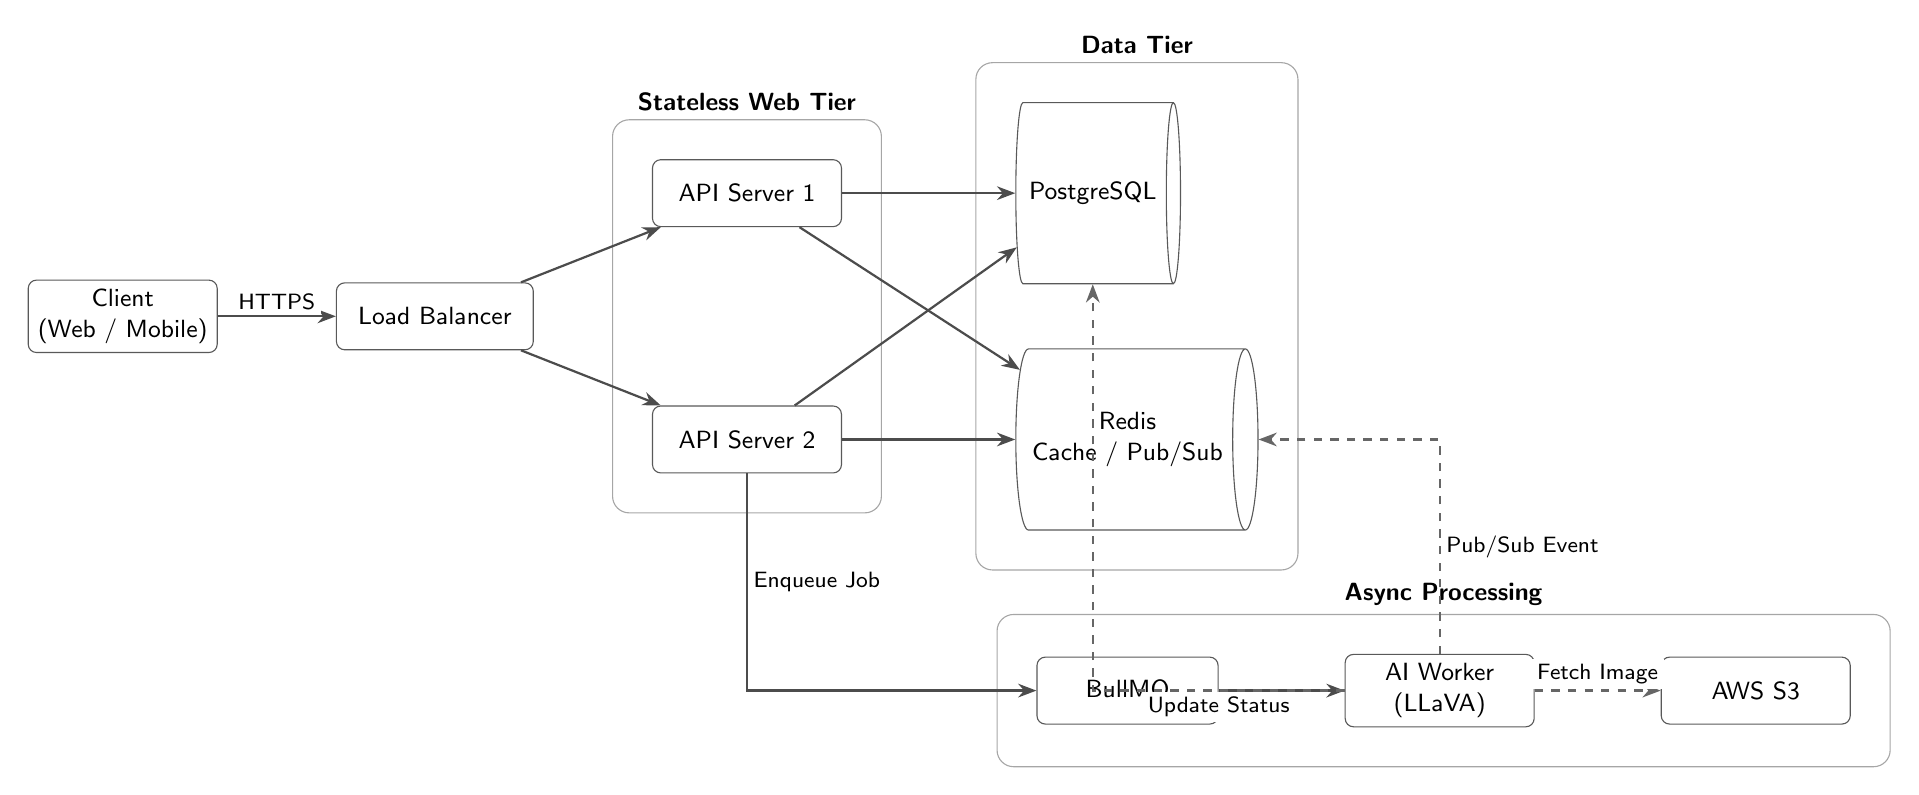
\begin{tikzpicture}[
    >=Stealth,
    node distance=1.4cm and 1.6cm,
    % -------------------------------------------------
    % Node styles
    % -------------------------------------------------
    component/.style={
        rectangle,
        rounded corners=3pt,
        draw=black!65,
        fill=white,
        minimum width=2.4cm,
        minimum height=0.85cm,
        align=center,
        font=\sffamily\small
    },
    loadbalancer/.style={
        rectangle,
        rounded corners=3pt,
        draw=black!65,
        fill=white,
        minimum width=2.5cm,
        minimum height=0.85cm,
        align=center,
        font=\sffamily\small
    },
    database/.style={
        cylinder,
        cylinder uses custom fill,
        cylinder body fill=white,
        cylinder end fill=white,
        draw=black!65,
        minimum width=2.3cm,
        minimum height=1.05cm,
        aspect=0.35,
        align=center,
        font=\sffamily\small
    },
    queue/.style={
        rectangle,
        rounded corners=3pt,
        draw=black!65,
        fill=white,
        minimum width=2.3cm,
        minimum height=0.85cm,
        align=center,
        font=\sffamily\small
    },
    % -------------------------------------------------
    % Tier containers
    % -------------------------------------------------
    tier/.style={
        rectangle,
        rounded corners=6pt,
        draw=black!35,
        inner sep=0.5cm
    },
    tierlabel/.style={
        font=\sffamily\bfseries\small,
        fill=white,
        inner sep=3pt
    },
    % -------------------------------------------------
    % Connections
    % -------------------------------------------------
    arrow/.style={
        ->,
        thick,
        draw=black!70
    },
    dashedarrow/.style={
        ->,
        dashed,
        thick,
        draw=black!60
    },
    edgelabel/.style={
        font=\sffamily\footnotesize,
        fill=white,
        inner sep=2pt
    }
]

% =====================================================
% External Client
% =====================================================

\node[component] (client) {Client\\(Web / Mobile)};

% =====================================================
% Load Balancer
% =====================================================

\node[loadbalancer, right=1.5cm of client] (lb)
    {Load Balancer};

% =====================================================
% Stateless Web Tier
% =====================================================

\node[component, above right=0.7cm and 1.5cm of lb] (api1)
    {API Server 1};

\node[component, below right=0.7cm and 1.5cm of lb] (api2)
    {API Server 2};

\node[tier,
      fit=(api1) (api2),
    label={[tierlabel]above:Stateless Web Tier}] (webtier) {};

% =====================================================
% Data Tier
% =====================================================

\node[database, right=2.2cm of api1] (postgres)
    {PostgreSQL};

\node[database, right=2.2cm of api2] (redis)
    {Redis\\Cache / Pub/Sub};

\node[tier,
      fit=(postgres) (redis),
    label={[tierlabel]above:Data Tier}] (datatier) {};

% =====================================================
% Asynchronous Processing
% =====================================================

\node[queue, below=1.6cm of redis] (bullmq)
    {BullMQ};

\node[component, right=1.6cm of bullmq] (worker)
    {AI Worker\\(LLaVA)};

\node[component, right=1.6cm of worker] (s3)
    {AWS S3};

\node[tier,
      fit=(bullmq) (worker) (s3),
    label={[tierlabel]above:Async Processing}] (asynctier) {};

% =====================================================
% Main Request Flow
% =====================================================

\draw[arrow]
    (client) -- node[edgelabel, above]{HTTPS} (lb);

\draw[arrow]
    (lb) -- (api1);

\draw[arrow]
    (lb) -- (api2);

% =====================================================
% API → PostgreSQL
% =====================================================

\draw[arrow]
    (api1) -- (postgres);

\draw[arrow]
    (api2) -- (postgres);

% =====================================================
% API → Redis
% =====================================================

\draw[arrow]
    (api1) -- (redis);

\draw[arrow]
    (api2) -- (redis);

% =====================================================
% Async Job Flow
% =====================================================

\draw[arrow]
    (api2) |- node[
        edgelabel,
        pos=0.25,
        right
    ]{Enqueue Job} (bullmq);

\draw[arrow]
    (bullmq) -- (worker);

% =====================================================
% Worker → S3
% =====================================================

\draw[dashedarrow]
    (worker) -- node[
        edgelabel,
        above
    ]{Fetch Image} (s3);

% =====================================================
% Worker → PostgreSQL
% =====================================================

\draw[dashedarrow]
    (worker) -| node[
        edgelabel,
        pos=0.25,
        below
    ]{Update Status} (postgres);

% =====================================================
% Worker → Redis
% =====================================================

\draw[dashedarrow]
    (worker) |- node[
        edgelabel,
        pos=0.25,
        right
    ]{Pub/Sub Event} (redis);

\end{tikzpicture}
\end{center}

\newpage

\section{Architectural Decisions \& Complexities}

The backend relies on several specific design choices to optimize for scalability, cost, and the unique constraints of local Large Language Models (LLMs).

\begin{itemize}
    \item \textbf{Stateless Web Tier via Encrypted Chat Context (Innovation):} 
    Traditional chat applications utilize stateful servers (binding a user to a specific server via WebSockets/sticky sessions) to maintain conversational memory. To keep our web tier completely stateless and horizontally scalable, we implemented a cryptographic context-passing innovation. 
    \begin{itemize}
        \item The AI agent's conversation summary and recent message array are encrypted using \texttt{A256GCM} on the server and sent to the client.
        \item The client stores this token and passes it back on the next request. 
        \item \textit{Justification:} This forces the LLM context to live client-side securely, completely eliminating server-side memory bottlenecks and allowing any API server to seamlessly pick up the conversation.
    \end{itemize}

    \item \textbf{Redis for Caching and Pub/Sub Messaging:}
    \begin{itemize}
        \item \textbf{Caching:} Daily macro aggregates are stored using Redis Hashes. Operations utilize \texttt{hIncrByFloat} for thread-safe, atomic increments, providing $O(1)$ read complexity for the dashboard, drastically reducing relational database load.
        \item \textbf{Pub/Sub Model:} We utilize Redis Pub/Sub to solve the asynchronous communication gap between the background AI workers and the stateless API servers. When a BullMQ worker finishes processing a vision task, it publishes a completion event to Redis. Subscribed API servers instantly receive this event and can push real-time Server-Sent Events (SSE) to the client, entirely avoiding inefficient database polling.
    \end{itemize}

    \item \textbf{Asynchronous Processing for Vision AI (BullMQ):}
    \begin{itemize}
        \item Local vision model inference (LLaVA) takes 10--30 seconds. Synchronous execution would block the Node.js event loop and trigger HTTP timeouts.
        \item \textit{Justification:} Event-driven decoupling. The API instantly returns a HTTP 202 (Accepted) with a \texttt{jobId}, while BullMQ manages retries, failure states, and concurrency limits for the GPU-bound workers safely in the background.
    \end{itemize}

    \item \textbf{Secure S3-to-Local Data Pipeline:}
    \begin{itemize}
        \item Local LLMs lack the native architecture to securely resolve remote AWS S3 URIs. 
        \item \textit{Justification:} The worker acts as a secure proxy. It downloads the S3 image to local \texttt{/temp}, converts it to Base64 for the LLM, and immediately deletes both the S3 object and local file upon completion. This strict ephemeral storage strategy guarantees user privacy and minimizes cloud storage costs.
    \end{itemize}

    \item \textbf{Relational Database (PostgreSQL):}
    \begin{itemize}
        \item \textit{Justification:} Nutrition logging requires complex, paginated time-range queries and aggregate mathematical functions (\texttt{SUM}). NoSQL data stores handle long-tail random access poorly when complex relations are required. PostgreSQL natively supports the ACID transactions required for accurate macro tracking.
    \end{itemize}
\end{itemize}

\newpage

\section{AI Agent Orchestration (LangGraph)}

A standard ReAct (Reasoning and Acting) loop fails frequently on smaller local models (e.g., Llama 3.1 8B) due to high cognitive load, resulting in infinite tool-calling loops and dropped parameters. To mitigate this, we implemented a \textbf{Supervisor Orchestrator Pattern}.

\vspace{1em}
\begin{center}
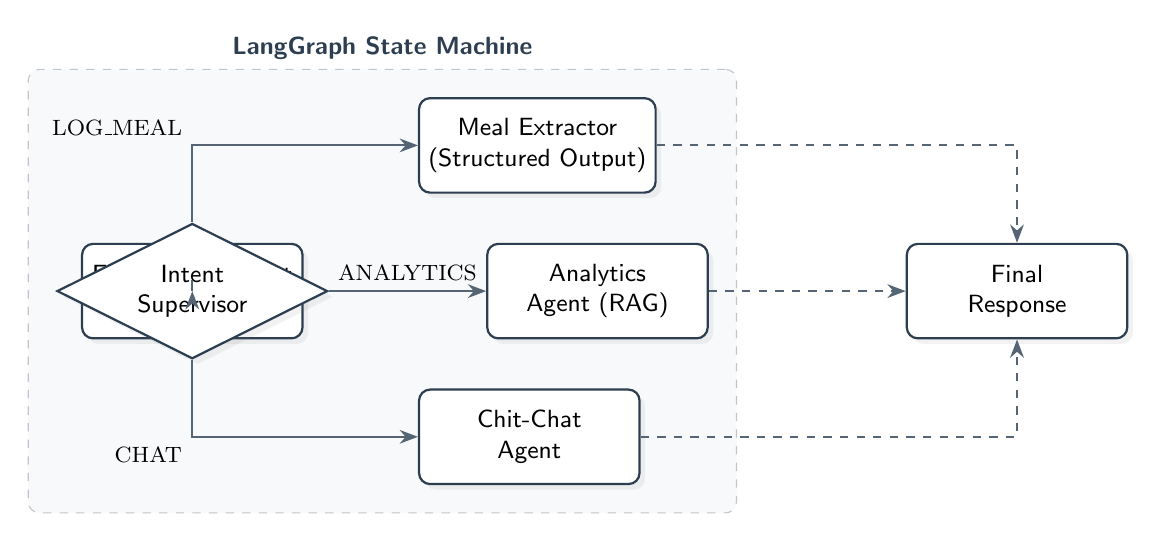
\begin{tikzpicture}[node distance=1.2cm and 2.5cm]

% Nodes
\node[component] (input) {Encrypted Context\\+ User Query};
\node[router] (supervisor) {Intent\\Supervisor};
\node[component, above right=0.8cm and 2cm of supervisor] (meal) {Meal Extractor\\(Structured Output)};
\node[component, right=2cm of supervisor] (analytics) {Analytics\\Agent (RAG)};
\node[component, below right=0.8cm and 2cm of supervisor] (chitchat) {Chit-Chat\\Agent};
\node[component, right=2.5cm of analytics] (output) {Final\\Response};

% Routing
\draw[arrow] (input) -- (supervisor);
\draw[arrow] (supervisor) |- node[above left, font=\footnotesize] {LOG\_MEAL} (meal);
\draw[arrow] (supervisor) -- node[above, font=\footnotesize] {ANALYTICS} (analytics);
\draw[arrow] (supervisor) |- node[below left, font=\footnotesize] {CHAT} (chitchat);

\draw[dashed_arrow] (meal) -| (output);
\draw[dashed_arrow] (analytics) -- (output);
\draw[dashed_arrow] (chitchat) -| (output);

% Background
\begin{scope}[on background layer]
    \node[group, fit=(supervisor) (meal) (analytics) (chitchat)] (graph) {};
    \node[above, font=\sffamily\bfseries\small, text=primary] at (graph.north) {LangGraph State Machine};
\end{scope}

\end{tikzpicture}
\end{center}

\subsection{Orchestration Logic}
\begin{itemize}
    \item \textbf{Intent Routing:} The Supervisor node utilizes \texttt{withStructuredOutput} to deterministically classify the user's intent. The LLM does not execute tools; it purely routes.
    \item \textbf{Domain Isolation:} By routing to specialized sub-agents, the system drastically shrinks the prompt size and cognitive load for each task. The \textit{Meal Extractor} forces JSON generation bypassing conversational text entirely, guaranteeing correct database insertion.
    \item \textbf{Psychological Circuit Breakers:} To prevent LangGraph recursion limits (ping-ponging), the Supervisor prompt contains dynamic stop-conditions: \textit{"If the last message in history is an AI confirmation, output FINISH."}
\end{itemize}

\newpage

\section{API Endpoints}

The backend exposes a RESTful API, completely decoupled from the frontend, supporting JSON payloads and Bearer Token authorization.

\subsection{Core Nutrition \& Aggregation}
All listing APIs support standard pagination (\texttt{limit}, \texttt{page}) and specific time-range query parameters.

\vspace{0.5em}
\begin{tabularx}{\textwidth}{>{\bfseries}l >{\ttfamily}l X}
\toprule
Method & Endpoint & Description \\
\midrule
GET & /nutrition/entries & Retrieves paginated food entries. Filterable via \texttt{startDate}, \texttt{endDate}, and \texttt{mealType}. \\
POST & /nutrition/entries & Creates a new food entry, executes SQL insert, and increments the daily Redis Hash atomically. \\
DELETE & /nutrition/entries/:id & Hard deletes an entry and recalculates the daily Redis cache. \\
GET & /nutrition/reports/weekly & Returns a 7-day chronological aggregation of Calories, Protein, Carbs, and Fat for chart rendering. \\
\bottomrule
\end{tabularx}

\subsection{AI \& Asynchronous Jobs}
\vspace{0.5em}
\begin{tabularx}{\textwidth}{>{\bfseries}l >{\ttfamily}l X}
\toprule
Method & Endpoint & Description \\
\midrule
POST & /uploads/presigned-url & Generates a secure, temporary AWS S3 pre-signed URL for direct client-to-cloud image uploads, saving API bandwidth. \\
GET & /jobs/:jobId & Polls Redis for the execution status of a BullMQ vision task (Pending, Completed, Failed). \\
POST & /agent/chat & Accepts the \texttt{encryptedContext} token and user prompt. Streams real-time Server-Sent Events (SSE) back to the client. \\
\bottomrule
\end{tabularx}

\end{document}